% This file was created by tikzplotlib v0.9.8.
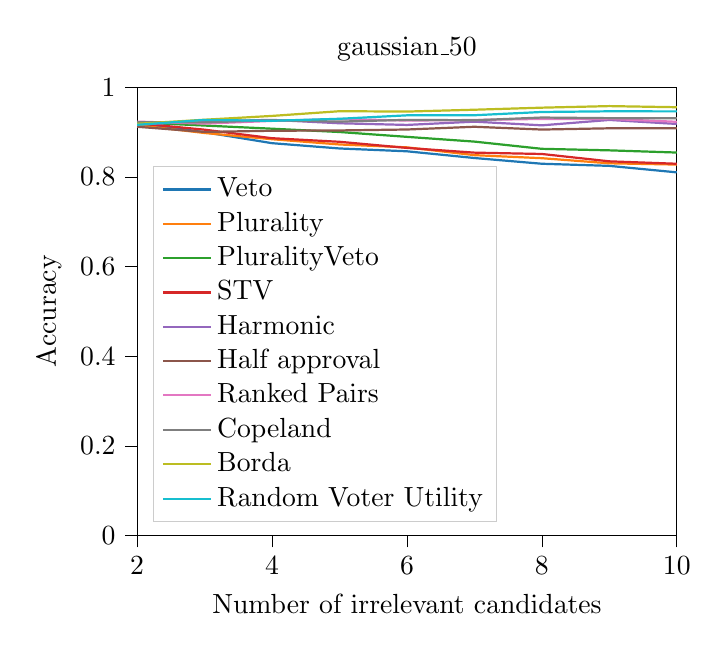
\begin{tikzpicture}

\definecolor{color0}{rgb}{0.12156862745098,0.466666666666667,0.705882352941177}
\definecolor{color1}{rgb}{1,0.498039215686275,0.0549019607843137}
\definecolor{color2}{rgb}{0.172549019607843,0.627450980392157,0.172549019607843}
\definecolor{color3}{rgb}{0.83921568627451,0.152941176470588,0.156862745098039}
\definecolor{color4}{rgb}{0.580392156862745,0.403921568627451,0.741176470588235}
\definecolor{color5}{rgb}{0.549019607843137,0.337254901960784,0.294117647058824}
\definecolor{color6}{rgb}{0.890196078431372,0.466666666666667,0.76078431372549}
\definecolor{color7}{rgb}{0.737254901960784,0.741176470588235,0.133333333333333}
\definecolor{color8}{rgb}{0.0901960784313725,0.745098039215686,0.811764705882353}

\begin{axis}[
legend cell align={left},
legend style={
  fill opacity=0.8,
  draw opacity=1,
  text opacity=1,
  at={(0.03,0.03)},
  anchor=south west,
  draw=white!80!black
},
tick align=outside,
tick pos=left,
title={gaussian\_50},
x grid style={white!69.0196078431373!black},
xlabel={Number of irrelevant candidates},
xmin=2, xmax=10,
xtick style={color=black},
y grid style={white!69.0196078431373!black},
ylabel={Accuracy},
ymin=0, ymax=1,
ytick style={color=black}
]
\addplot [thick, color0]
table {%
2 0.9194
3 0.8995
4 0.875
5 0.8632
6 0.8569
7 0.8419
8 0.8291
9 0.8244
10 0.8099
};
\addlegendentry{Veto}
\addplot [thick, color1]
table {%
2 0.9152
3 0.8977
4 0.8838
5 0.8721
6 0.8657
7 0.8483
8 0.8415
9 0.8301
10 0.8273
};
\addlegendentry{Plurality}
\addplot [thick, color2]
table {%
2 0.9213
3 0.9143
4 0.9073
5 0.8999
6 0.8891
7 0.8785
8 0.8624
9 0.859
10 0.8541
};
\addlegendentry{PluralityVeto}
\addplot [thick, color3]
table {%
2 0.9195
3 0.9051
4 0.8861
5 0.8781
6 0.8644
7 0.8539
8 0.8509
9 0.8345
10 0.8291
};
\addlegendentry{STV}
\addplot [thick, color4]
table {%
2 0.9166
3 0.9237
4 0.927
5 0.9194
6 0.9157
7 0.923
8 0.9148
9 0.9268
10 0.9179
};
\addlegendentry{Harmonic}
\addplot [thick, color5]
table {%
2 0.9116
3 0.9001
4 0.9027
5 0.9034
6 0.9055
7 0.9116
8 0.9054
9 0.9082
10 0.9084
};
\addlegendentry{Half approval}
\addplot [thick, color6]
table {%
2 0.9231
3 0.9186
4 0.9247
5 0.9289
6 0.9254
7 0.9267
8 0.9291
9 0.9291
10 0.9227
};
\addlegendentry{Ranked Pairs}
\addplot [thick, white!49.8039215686275!black]
table {%
2 0.9215
3 0.9214
4 0.9261
5 0.9231
6 0.927
7 0.9261
8 0.9322
9 0.9308
10 0.9308
};
\addlegendentry{Copeland}
\addplot [thick, color7]
table {%
2 0.9182
3 0.9273
4 0.9358
5 0.9463
6 0.9455
7 0.9496
8 0.9542
9 0.9577
10 0.9552
};
\addlegendentry{Borda}
\addplot [thick, color8]
table {%
2 0.9159
3 0.9269
4 0.9249
5 0.9294
6 0.9371
7 0.9373
8 0.9446
9 0.9461
10 0.9459
};
\addlegendentry{Random Voter Utility}
\end{axis}

\end{tikzpicture}
